\documentclass[12pt, a4paper, oneside]{ctexart}

\usepackage{amsmath, amsthm, amssymb, mathrsfs, graphicx}
\usepackage{tcolorbox, hyperref, enumerate}

% hw-preamble.tex

% geometry for A4 paper
% See https://tex.stackexchange.com/a/119912/23098
\geometry{
  left=20.0mm,
  top=20.0mm,
  bottom=20.0mm,
  textwidth=130mm, % main text block
  marginparsep=5.0mm, % gutter between main text block and margin notes
  marginparwidth=50.0mm % width of margin notes
}

% for colors
\usepackage{xcolor} % usage: \color{red}{text}
% predefined colors
\newcommand{\red}[1]{\textcolor{red}{#1}} % usage: \red{text}
\newcommand{\blue}[1]{\textcolor{blue}{#1}}
\newcommand{\teal}[1]{\textcolor{teal}{#1}}

\usepackage{todonotes}

% heading
\usepackage{sectsty}
\setcounter{secnumdepth}{2}
\allsectionsfont{\centering\huge\rmfamily}

% for Chinese
\usepackage{xeCJK}
\usepackage{zhnumber}
\setCJKmainfont[BoldFont=FandolSong-Bold.otf]{FandolSong-Regular.otf}

% for fonts
\usepackage{fontspec}
\newcommand{\song}{\CJKfamily{song}} 
\newcommand{\kai}{\CJKfamily{kai}} 

% To fix the ``MakeTextLowerCase'' bug:
% See https://github.com/Tufte-LaTeX/tufte-latex/issues/64#issuecomment-78572017
% Set up the spacing using fontspec features
\renewcommand\allcapsspacing[1]{{\addfontfeature{LetterSpace=15}#1}}
\renewcommand\smallcapsspacing[1]{{\addfontfeature{LetterSpace=10}#1}}

% for url
\usepackage{hyperref}
\hypersetup{colorlinks = true, 
  linkcolor = teal,
  urlcolor  = teal,
  citecolor = blue,
  anchorcolor = blue}

\newcommand{\me}[4]{
    \author{
      {\bfseries 姓名:}\underline{#1}\hspace{2em}
      {\bfseries 学号:}\underline{#2}\hspace{2em}\\[10pt]
      {\bfseries 评分:}\underline{#3\hspace{3em}}\hspace{2em}
      {\bfseries 评阅:}\underline{#4\hspace{3em}}
  }
}

% Please ALWAYS Keep This.
\newcommand{\noplagiarism}{
  \begin{center}
    \fbox{\begin{tabular}{@{}c@{}}
      请独立完成作业,不得抄袭。\\
      若得到他人帮助, 请致谢。\\
      若参考了其它资料,请给出引用。\\
      鼓励讨论,但需独立书写解题过程。
    \end{tabular}}
  \end{center}
}

\newcommand{\goal}[1]{
  \begin{center}{\fcolorbox{blue}{yellow!60}{\parbox{0.50\textwidth}{\large 
    \begin{itemize}
      \item 体会``思维的乐趣''
      \item 初步了解递归与数学归纳法 
      \item 初步接触算法概念与问题下界概念
    \end{itemize}}}}
  \end{center}
}

% Each hw consists of four parts:
\newcommand{\beginrequired}{\hspace{5em}\section{作业 (必做部分)}}
\newcommand{\beginoptional}{\section{作业 (选做部分)}}
\newcommand{\beginot}{\section{Open Topics}}
\newcommand{\begincorrection}{\section{订正}}
\newcommand{\beginfb}{\section{反馈}}

% for math
\usepackage{amsmath, mathtools, amsfonts, amssymb}
\newcommand{\set}[1]{\{#1\}}

% define theorem-like environments
\usepackage[amsmath, thmmarks]{ntheorem}

\theoremstyle{break}
\theorempreskip{2.0\topsep}
\theorembodyfont{\song}
\theoremseparator{}
\newtheorem{problem}{题目}[subsection]
\renewcommand{\theproblem}{\arabic{problem}}
\newtheorem{ot}{Open Topics}

\theorempreskip{3.0\topsep}
\theoremheaderfont{\kai\bfseries}
\theoremseparator{:}
\theorempostwork{\bigskip\hrule}
\newtheorem*{solution}{解答}
\theorempostwork{\bigskip\hrule}
\newtheorem*{revision}{订正}

\theoremstyle{plain}
\newtheorem*{cause}{错因分析}
\newtheorem*{remark}{注}

\theoremstyle{break}
\theorempostwork{\bigskip\hrule}
\theoremsymbol{\ensuremath{\Box}}
\newtheorem*{proof}{证明}

% \newcommand{\ot}{\blue{\bf [OT]}}

% for figs
\renewcommand\figurename{图}
\renewcommand\tablename{表}

% for fig without caption: #1: width/size; #2: fig file
\newcommand{\fig}[2]{
  \begin{figure}[htbp]
    \centering
    \includegraphics[#1]{#2}
  \end{figure}
}
% for fig with caption: #1: width/size; #2: fig file; #3: caption
\newcommand{\figcap}[3]{
  \begin{figure}[htbp]
    \centering
    \includegraphics[#1]{#2}
    \caption{#3}
  \end{figure}
}
% for fig with both caption and label: #1: width/size; #2: fig file; #3: caption; #4: label
\newcommand{\figcaplbl}[4]{
  \begin{figure}[htbp]
    \centering
    \includegraphics[#1]{#2}
    \caption{#3}
    \label{#4}
  \end{figure}
}
% for margin fig without caption: #1: width/size; #2: fig file
\newcommand{\mfig}[2]{
  \begin{marginfigure}
    \centering
    \includegraphics[#1]{#2}
  \end{marginfigure}
}
% for margin fig with caption: #1: width/size; #2: fig file; #3: caption
\newcommand{\mfigcap}[3]{
  \begin{marginfigure}
    \centering
    \includegraphics[#1]{#2}
    \caption{#3}
  \end{marginfigure}
}

\usepackage{fancyvrb}

% for algorithms
\usepackage[]{algorithm}
\usepackage[]{algpseudocode} % noend
% See [Adjust the indentation whithin the algorithmicx-package when a line is broken](https://tex.stackexchange.com/a/68540/23098)
\newcommand{\algparbox}[1]{\parbox[t]{\dimexpr\linewidth-\algorithmicindent}{#1\strut}}
\newcommand{\hStatex}[0]{\vspace{5pt}}
\makeatletter
\newlength{\trianglerightwidth}
\settowidth{\trianglerightwidth}{$\triangleright$~}
\algnewcommand{\LineComment}[1]{\Statex \hskip\ALG@thistlm \(\triangleright\) #1}
\algnewcommand{\LineCommentCont}[1]{\Statex \hskip\ALG@thistlm%
  \parbox[t]{\dimexpr\linewidth-\ALG@thistlm}{\hangindent=\trianglerightwidth \hangafter=1 \strut$\triangleright$ #1\strut}}
\makeatother

% for footnote/marginnote
% see https://tex.stackexchange.com/a/133265/23098
\usepackage{tikz}
\newcommand{\circled}[1]{%
  \tikz[baseline=(char.base)]
  \node [draw, circle, inner sep = 0.5pt, font = \tiny, minimum size = 8pt] (char) {#1};
}
\renewcommand\thefootnote{\protect\circled{\arabic{footnote}}}

\title{\vspace{-2em}\textbf{第0讲:\LaTeX}}
\me{李四}{210000000}{}{}
\date{\today}

\begin{document}

\maketitle
\section*{Problem 1}
\begin{problem}
证明:
$$
  Pr(\bigcup_{i=1}^n A_i) \leq \sum_{i=1}^n Pr(A_i)
$$
\end{problem}

\begin{proof}
  概率空间的定义:非负性和可加性。

  首先,证明一个性质$$P(A\cup B) \leq P(A) + P(B)$$(事件的并概率上界)

  设两个相交的事件,即A和B。

  可知$A \cup B = A\cup (A^c \cap B), B=(A\cap B)\cup (A^c \cap B)$

  由可加性可知:

  $$P(A\ cup B) = P(A)+P(A^c \cap B)$$
  $$P(B) = P(A\cap B) + P(A^c\cap B)$$

  $$\Rightarrow P(A \cup B) = P(A)+P(B) - P(A \cap B)$$

  由非负性可知, $$P(A \cup B) \leq P(A)+P(B)$$

  至此证成事件的并概率上界性质;

  可以将此性质用于$A_1$和$A_2\cup A_3 \cup ... \cup A_n$

  $$Pr(A_1) \cup Pr(A_2\cup A_3 \cup ... \cup A_n) \leq Pr(A_1) + Pr(A_2\cup A_3 \cup ... \cup A_n)$$

  再用此方法计算$Pr(A_2)$和$Pr(A_3\cup A_4 \cup ... \cup A_n)$;

  得到$$Pr(A_2) \cup Pr(A_3\cup A_4 \cup ... \cup A_n) \leq Pr(A_2) + Pr(A_3\cup A_4 \cup ... \cup A_n)$$

  以此类推,可得

  $$\Rightarrow Pr(A_1 \cup A_2 \cup .. \cup A_n) \leq Pr(A_1) + Pr(A_2) + ... + Pr(A_n)$$
  即
  $$Pr(\bigcup_{i=1}^n A_i) \leq \sum_{i=1}^n Pr(A_i)
  $$
\end{proof}


\begin{problem}
[Principle of Inclusion and Exclusion (PIE)] Prove that
$\mathbf{Pr}\left( \bigcup_{i=1}^n A_i\right) = \sum_{\emptyset \neq S \subseteq [n]} (-1)^{|S|-1} \mathbf{Pr}\left( \bigcap_{i \in S} A_i \right) $
, where$ [n]=\{1,2,\ldots,n\} $.
\end{problem}

\begin{proof}

  将用数学归纳法证明.

  Consider a single set $A_1$. Then the principle of inclusion-exclusion states that $|A_1| = |A_1| + | A_1 | - | A_1 \cap A_1 | = | A_1 |$, which is trivially true. Now consider a collection of exactly two sets $A$ and $B$. Then $|A \cup B| = |A| + |B| - |A \cap B|$. Assume that the principle of inclusion-exclusion holds for unions of $n$ terms. By grouping terms, and simplifying some of them, the principle can be deduced for unions of $n+1$ terms⁴.

  Therefore, $\mathbf{Pr}\left( \bigcup_{i=1}^n A_i\right) = \sum_{\emptyset \neq S \subseteq [n]} (-1)^{|S|-1} \mathbf{Pr}\left( \bigcap_{i \in S} A_i \right) $, where $[n]=\{1,2,\ldots,n\}$.


\end{proof}

\begin{note}
  无论 \textbackslash itemlize 还是\textbackslash enumerate 中的 \textbackslash item 都支持一个可选参数以临时更换列表标志(即无序列表前的点或有序列表前的 ``1.'')。
  此外,使用 \textbackslash enumerate 的可选参数也可以改变有序列表的图标。当然,这些列表是可以嵌套的。
\end{note}

\begin{problem}
请用 \LaTeX 输出下图中的公式。

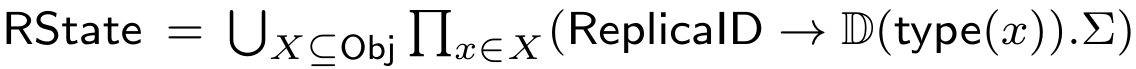
\includegraphics[width=1\textwidth]{figs/formula}
\end{problem}

\begin{solution}

\end{solution}

\begin{note}
  当你不认识某些数学符号的时候,你可以使用 \href{http://detexify.kirelabs.org/classify.html}{Detexify} 或 \href{https://mathpix.com/}{mathpix} 等工具进行识别。
  你也可以使用 \href{https://latex.codecogs.com/legacy/eqneditor/editor.php}{Online LaTeX Equation Editor} 或者你编辑器中的符号表进行输入。
\end{note}

\begin{problem}
请用 \LaTeX 输出下图中的表格。

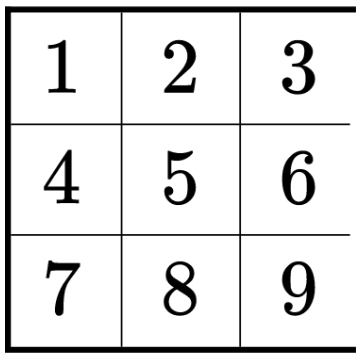
\includegraphics[width=.3\textwidth]{figs/table}
\end{problem}

\begin{solution}

\end{solution}

\begin{note}
  如果你觉得 \LaTeX 的表格填起来太麻烦,你也可以使用 \href{https://www.tablesgenerator.com/}{TablesGenerator} 帮你生成。
\end{note}

\begin{problem}
(此部分为选做)本学期还有可能需要你编写一些伪代码,\LaTeX 中当然有相应的宏包—— \href{http://tug.ctan.org/macros/latex/contrib/algorithmicx/algorithmicx.pdf}{algorithmicx} 。

请用 \LaTeX 输出下图中的算法。

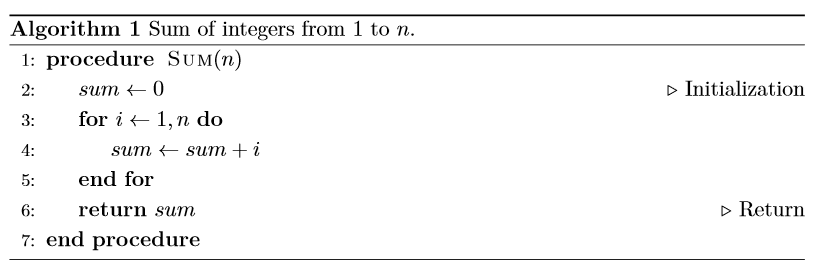
\includegraphics[width=\textwidth]{figs/algorithm}
\end{problem}

\begin{solution}

\end{solution}

\end{document}